%\documentclass[honours,12pt,twoside]{unswthesis}

\usepackage{afterpage}
\usepackage{amsfonts}
\usepackage{amsmath}
\usepackage{amssymb}
\usepackage{amsthm}
\usepackage[english]{babel}
\usepackage{graphicx}
\usepackage{natbib}
\usepackage[utf8]{inputenc}
\usepackage{latexsym}
\usepackage{url}
\usepackage{todonotes}
\usepackage{tikz}
\usepackage{pdfpages}
\usetikzlibrary{arrows}
\usepackage{float}

\usepackage{booktabs}
\renewcommand{\arraystretch}{1.2}


%%%%%%%%%%%%%%%%%%%%%%%%%%%%%%%%%%%%%%%%%%%%%%%%%%%%%%%%%%%%%%%%%
%
%  The following are some simple LaTeX macros to give some
%  commonly used letters in funny fonts. You may need more or less of
%  these
%
\newcommand{\R}{\mathbb{R}}
\newcommand{\Q}{\mathbb{Q}}
\newcommand{\C}{\mathbb{C}}
\newcommand{\N}{\mathbb{N}}
\newcommand{\F}{\mathbb{F}}
\newcommand{\PP}{\mathbb{P}}
\newcommand{\T}{\mathbb{T}}
\newcommand{\Z}{\mathbb{Z}}
\newcommand{\B}{\mathfrak{B}}
\newcommand{\BB}{\mathcal{B}}
\newcommand{\M}{\mathfrak{M}}
\newcommand{\X}{\mathfrak{X}}
\newcommand{\Y}{\mathfrak{Y}}
\newcommand{\CC}{\mathcal{C}}
\newcommand{\E}{\mathbb{E}}
\newcommand{\cP}{\mathcal{P}}
\newcommand{\cS}{\mathcal{S}}
\newcommand{\A}{\mathcal{A}}
\newcommand{\ZZ}{\mathcal{Z}}

%%%%%%%%%%%%%%%%%%%%%%%%%%%%%%%%%%%%%%%%%%%%%%%%%%%%%%%%%%%%%%%%%%%%%
%
% The following are much more esoteric commands that I have left in
% so that this file still processes. Use or delete as you see fit
%
\newcommand{\bv}[1]{\mbox{BV($#1$)}}
\newcommand{\comb}[2]{\left(\!\!\!\begin{array}{c}#1\\#2\end{array}\!\!\!\right)
}
\newcommand{\Lat}{{\rm Lat}}
\newcommand{\var}{\mathop{\rm var}}
\newcommand{\Pt}{{\mathcal P}}
\def\tr(#1){{\rm trace}(#1)}
\def\Exp(#1){{\mathbb E}(#1)}
\def\Exps(#1){{\mathbb E}\sparen(#1)}
\newcommand{\floor}[1]{\left\lfloor #1 \right\rfloor}
\newcommand{\ceil}[1]{\left\lceil #1 \right\rceil}
\newcommand{\hatt}[1]{\widehat #1}
\newcommand{\modeq}[3]{#1 \equiv #2 \,(\text{mod}\, #3)}
\newcommand{\rmod}{\,\mathrm{mod}\,}
\newcommand{\p}{\hphantom{+}}
\newcommand{\vect}[1]{\mbox{\boldmath $ #1 $}}
\newcommand{\reff}[2]{\ref{#1}.\ref{#2}}
\newcommand{\psum}[2]{\sum_{#1}^{#2}\!\!\!'\,\,}
\newcommand{\bin}[2]{\left( \begin{array}{@{}c@{}}
				#1 \\ #2
			\end{array}\right)	}
%
%  Macros - some of these are in plain TeX (gasp!)
%
\newcommand{\be}{($\beta$)}
\newcommand{\eqp}{\mathrel{{=}_p}}
\newcommand{\ltp}{\mathrel{{\prec}_p}}
\newcommand{\lep}{\mathrel{{\preceq}_p}}
\def\brack#1{\left \{ #1 \right \}}
\def\bul{$\bullet$\ }
\def\cl{{\rm cl}}
\let\del=\partial
\def\enditem{\par\smallskip\noindent}
\def\implies{\Rightarrow}
\def\inpr#1,#2{\t \hbox{\langle #1 , #2 \rangle} \t}
\def\ip<#1,#2>{\langle #1,#2 \rangle}
\def\lp{\ell^p}
\def\maxb#1{\max \brack{#1}}
\def\minb#1{\min \brack{#1}}
\def\mod#1{\left \vert #1 \right \vert}
\def\norm#1{\left \Vert #1 \right \Vert}
\def\paren(#1){\left( #1 \right)}
\def\qed{\hfill \hbox{$\Box$} \smallskip}
\def\sbrack#1{\Bigl \{ #1 \Bigr \} }
\def\ssbrack#1{ \{ #1 \} }
\def\smod#1{\Bigl \vert #1 \Bigr \vert}
\def\smmod#1{\bigl \vert #1 \bigr \vert}
\def\ssmod#1{\vert #1 \vert}
\def\sspmod#1{\vert\, #1 \, \vert}
\def\snorm#1{\Bigl \Vert #1 \Bigr \Vert}
\def\ssnorm#1{\Vert #1 \Vert}
\def\sparen(#1){\Bigl ( #1 \Bigr )}

\newcommand\blankpage{%
    \null
    \thispagestyle{empty}%
    \addtocounter{page}{-1}%
    \newpage}
    
%%%%%%%%%%%%%%%%%%%%%%%%%%%%%%%%%%%%%%%%%%%%%%%%%%%%%%%%%%%%%%
%
% These environments allow you to get nice numbered headings
%  for your Theorems, Definitions etc.  
%
%  Environments
%
%%%%%%%%%%%%%%%%%%%%%%%%%%%%%%%

\newtheorem{theorem}{Theorem}[section]
\newtheorem{lemma}[theorem]{Lemma}
\newtheorem{proposition}[theorem]{Proposition}
\newtheorem{corollary}[theorem]{Corollary}
\newtheorem{conjecture}[theorem]{Conjecture}
\newtheorem{definition}[theorem]{Definition}
\newtheorem{example}{Example}
\newtheorem{remark}[theorem]{Remark}
\newtheorem{question}[theorem]{Question}
\newtheorem{notation}[theorem]{Notation}
\numberwithin{equation}{section}

%\begin{document}

\chapter{Neural networks}\label{neuralNets-intro}

To understand the models outlined in \textbf{Chapter}, it is necessary to introduce neural networks. This chapter covers the structure and workings behind basic neural networks.

% - Basic neural networks theory + perceptron
% - Loss functions
% - Minimisation functions
% 
% - Convolutional neural networks overview
% - Convolution layer
% - ReLU
% - Pooling
% - Fully connected layers
% 
% - 3D CNNs overview

Neural networks have become increasingly popular with the advancement of computing power. They have the ability to detect and utilise predictors and patterns that may not be easily employed using other statistical methods. Given enough data, computational power, and training time, neural network models have exhibited a high accuracy in solving complex problems. In some cases, recorded accuracies have been found to be higher than that of humans (see MNIST and ImageNET). They have been implemented in a number of commonplace technologies, such as face and voice recognition, language translation, and AI.

The construction of neural networks has to be conducted with some care, however. The resulting models are difficult to interpret, and are prone to overfitting. 

\section{Basic structure}\label{nnets-structure}

Neural networks are made up of a series of layers of \textit{neurons}, as shown in \textbf{Figure}. The first layer is an input layer, where data is fed into the model. The last layer is an output layer, generating the final result. The central layers are known as \textit{hidden layers}, which conduct most of the processing.

% Diagram of basic neural network structure. Input, 1 hidden layer and series of output layers
\begin{figure}[ht]
	\centering
	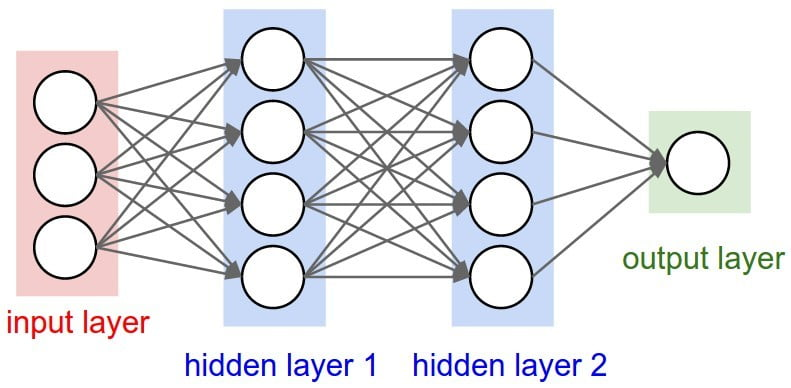
\includegraphics[width=\textwidth]{Images/3_nnet_structure.jpg}
	\caption{Basic neural network structure.}
	\small Image taken from \url{'https://www.digitaltrends.com/cool-tech/what-is-an-artificial-neural-network/'}
\end{figure}

Let $\mathbf{x} = (x_1, x_2, \ldots, x_n)^\top$ be a vector of $n$ input variables. Let $\mathbf{w} = (w_1, \ldots, w_n)^\top$ be a vector of weights, where each $w_i$ is associated with $x_i$. Let $b$ be an additional variable be added, known as the \textit{bias}. This bias is not to be confused with statistical bias. The output of a single neuron is given by
\[
	a = \sigma(\mathbf{w}\cdot\mathbf{x} + b),
\]
where $\sigma(\cdot)$ is some activation function and $a$ is known as an \textit{activation value}.

The weights and biases are chosen such that they minimise some \textit{cost function} $C(W,B)$, where $W$ is the set of all weights and $B$ the set of all biases in the neural network. However, as there can be a very large number of variables, it is not feasible to minimise $C(W,B)$ analytically.

Instead, this minimisation is approximated via the Gradient Descent algorithm \textbf{(see Section)}. This algorithm is run until the cost falls below a specified margin, or reaches a maximum number of iterations.

\section{Notation}\label{nnets-not}

In order to more efficiently and coherantly describe the computations, it is necessary to introduce some notation.

Define $\mathbf{w}_j^l$ to be the vector of weights used by the $j$th neuron of the $l$th layer, where $w_{ji}^l$ is the weight attributed to the $i$th neuron of the $(l-1)$th layer.

$b_j^l$ is the bias of the $j$th neuron in the $l$th layer.

$\mathbf{a}^l$ is the vector of activation values (outputs) for the $l$th layer, where $a_j^l$ is the activation value of the $j$th neuron of that layer.

Set $z_j^l = \mathbf{w}_j^l\cdot \mathbf{a}^{l-1} + b_j^l= \sum_k w_{jk}^la_k^{l-1} + b_j^l$ to be the values calculated before activation, and $\mathbf{z}^l$ to be the vector of $z_j^l$ for layer $l$. Set $Z$ to be the set of all $z_j^l$ in the whole network.

Let $L$ be the number of layers in the network so that $\mathbf{a}^L$ are the activation values of the final output layer.

Let $X = \{\mathbf{x}_1, \mathbf{x}_2, \ldots, \mathbf{x}_n\}$ be the set of $n$ training inputs. Let the responses be $Y = \{\mathbf{y}_1, \mathbf{y}_2, \ldots, \mathbf{y}_n\}$, with $y_{ij}$ the $j$th variable of $\mathbf{y}_i$.

Let $W$ and $B$ be the sets of all weights and biases as before.

Let $\eta$ be the learning rate of the minimiser during training.

\section{Activation functions}\label{nnets-act}

Activation functions serve to introduce nonlinearity into the model. 

For the perceptron, a basic neuron, we have the step function,
\[
	x_i \in \{0,1\} \text{ and } \sigma(z) = \begin{cases}
		1 & z > 0 \\
		0 & z \le 0
	\end{cases}.
\]

To allow for continuous outputs, other common activation functions include the sigmoid,
\[
	\sigma(z) = \dfrac{1}{1+e^{-z}},
\]
and tanh functions,
\[
	\sigma(z) = \tanh(z),
\]
which are smooth approximations to a step activation function.

Rectified Linear Unit (ReLU) activation is a common activation function for convolutional neural networks. It is given by,
\[
	\sigma(z) = \max(0, z),
\]
which allows for some neurons to output 0 and be essentially deactivated. Using ReLU activation helps to avoid the vanishing gradient problem, which can occur during gradient descent (\textbf{see Section}).

A common activation function for the final layer is the softmax function,
\[
	\sigma(z_j) = \dfrac{e^{z_j}}{\sum_ke^{z_k}}.
\]
This is used for classification tasks as the output takes on the form of a probability distribution.

\section{Cost functions}\label{nnets-cost}

Weights and biases are chosen such that they approximately minimise some cost function.

In using gradient descent \textbf{(see Section)}, there are two requirements. First, that the cost, $C_X(\cdot)$, accrued from all samples, $X$, can be expressed as the mean of costs accrued from $n$ distinct subsamples of $X$, denoted $X_i$,
\[
	C_X(W, B) = \dfrac{1}{n}\sum_{i=1}^n C_{X_i}(W,B).
\]

The second requirement is that the only activation values that the cost is dependent on are those in the final output layer of the network, $\mathbf{a}^L$.

There are a number of cost functions in frequent use, and the choice of cost function is dependent on the context of the problem.

One of the most common cost functions for regression is the quadratic cost, or Mean Squared Error cost, given by
\[
	C(W,B) = \dfrac{1}{2n}\sum_{i=1}^n||\mathbf{a}^L(\mathbf{x}_i,W,B) - \mathbf{y}_i ||^2,
\]
where $\|\cdot\|$ is the Euclidean norm. This form is convenient for backpropagation \textbf{(see Section)} as it has an efficiently computable gradient,
\[
	\nabla_aC = \dfrac{1}{n}\sum_{i=1}^n||\mathbf{a}^L(\mathbf{x}_i,W,B) - \mathbf{y}_i ||.
\]
In using quadratic cost, when there is a high amount of error, the learning rate is low.

The most common cost function for classification tasks is cross entropy, given by
\[
	C(W,B) = -\dfrac{1}{n}\sum_{i=1}^n\sum_j\big[y_{ij}\ln a_j^L(\mathbf{x}_i,W,B) + (1 - y_{ij})\ln (1 - a_j^L(\mathbf{x}_i,W,B))\big],
\]
with gradient
\[
	\nabla_aC = \dfrac{1}{n}\sum_{i=1}^n\sum_j\dfrac{a_j^L(\mathbf{x}_i,W,B) - y_{ij}}{a_j^L(\mathbf{x}_i,W,B)(1-a_j^L(\mathbf{x}_i,W,B))}.
\]
Unlike the quadratic cost, when error is high, the learning rate is also high.

%Cost functions can include: the quadratic (simple), cross-entropy, regularisation (L1, L2, dropout, artificial expansion of training data).
%In using cross-entropy, the learning rate of the weight is controlled by the amount of error. This is unlike the quadratic cost function, which has a very slow learning rate when there is high error.
%Changing these can improve a model.
%Other improvements made by making better initialisations of weights, and better heuristics to choose hyper-parameters.

\section{Gradient descent}\label{nnets-graddesc}

Weights and biases are chosen such that they will minimise the cost function. However, there are too many variables for this to be done analytically, and so they are instead estimated using the Gradient Descent algorithm.

As described by Nielson \cite{Nielson2015}, Gradient Descent works by considering the gradient of the cost given the current weights and biases. The algorithm then shifts the weights and biases by a small amount such that the cost will decrease. The amount that the values shift by is referred to as the learning rate, denoted $\eta$ as before.

For all weights and biases denoted $\mathbf{v}$, the change in cost $C(\mathbf{v})$ is given by
\begin{align*}
	\Delta C(\mathbf{v}) & \approx \dfrac{\partial C}{\partial v_1}\Delta v_1 + \dfrac{\partial C}{\partial v_2}\Delta v_2 + \cdots + \dfrac{\partial C}{\partial v_N}\Delta v_N\text{, for some number of variables } N\\
	& = \nabla C(\mathbf{v})\cdot \Delta \mathbf{v}.
\end{align*}

The next values of $\mathbf{v}$ are chosen such that the cost will decrease by an amount controlled by $\eta$, such that
\[
	\Delta\mathbf{v} = -\eta \nabla C(\mathbf{v}), \quad \text{ where }\eta > 0.
\]
By substitution, we can write
\[
	\Delta C(\mathbf{v}) \approx -\eta \|\nabla C(\mathbf{v})\|^2 \le 0,
\]
where $\|\cdot\|$ is the Euclidean norm.

Thus if the new $\mathbf{v}' = \mathbf{v} - \eta \nabla C(\mathbf{v})$, the cost will decrease.

In training a neural network, the size of the shift can be set to $\|\Delta\mathbf{v}\| = \epsilon$, for some $\epsilon > 0$. It can be shown that the $\Delta\mathbf{v}$ which gives the greatest decrease in $C(\mathbf{v})$ is a function of $\epsilon$ and $\nabla C$.

\begin{proposition}\label{nnets-graddescminproof}
	If the size of the shift is constrained such that $\|\Delta\mathbf{v}\| = \epsilon$ where $\epsilon > 0$, then $\nabla C \cdot \Delta\mathbf{v}$ is minimised by $\Delta\mathbf{v} = -\eta\nabla C$, where $\eta = \dfrac{\epsilon}{\|\nabla C\|}$.
\end{proposition}

\begin{proof}
	Using the Cauchy-Schwarz Inequality,
	\[
			|\nabla C\cdot\Delta\mathbf{v}| \le \|\nabla C\|\times\|\Delta\mathbf{v}\|.
	\]
	Then the minimum is given by, \begin{align*}
		\min(\nabla C\cdot\Delta\mathbf{v}) & = -\|\nabla C\|\times\|\Delta\mathbf{v}\| \\
		& = -\epsilon\|\nabla C\| \\
		& = -\dfrac{\epsilon\|\nabla C\|^2}{\|\nabla C\|} \\
		& = -\dfrac{\epsilon\nabla C\cdot\nabla C}{\|\nabla C\|}.
	\end{align*}
	Then by equating the coefficients of $\nabla C$,
	\begin{align*}
		\operatorname*{arg\,min}_{\Delta\mathbf{v}}(\nabla C\cdot\Delta\mathbf{v}) & = -\dfrac{\epsilon\nabla C}{\|\nabla C\|} \\
		& = -\eta\nabla C,\quad\eta = \dfrac{\epsilon}{\|\nabla C\|}.
	\end{align*}
\end{proof}

As gradient descent moves the coefficients in the direction of the steepest negative gradient, it assumes that the starting values are close enough to the global minimum to converge. If this assumption is not satistifed, the algorithm will instead converge to the local minimum. However, it is not possible to confirm whether the weights are converging to the global minimum or not.

%To address this, it is commonplace to initialise the weights randomly.
%
%A common distribution for initialising weights is the truncated normal distribution, which has the shape of the normal distribution $\mathcal{N}(\mu, \sigma^2)$, but is bounded such that $X\in(a,b),-\infty\le a < b\le \infty$.

As the updated weights and biases rely on the gradient, it should be noted that these gradients are then required to be significantly different from zero. When this is not the case, we have what is called the Vanishing Gradient Problem, which is discussed further in section \ref{nnet-vanishinggradprob}.

\subsection*{Stochastic gradient descent}\label{nnets-stochgraddesc}

As the neural network has a very large number of weights, gradient descent is a highly computationally intensive algorithm. To improve training time, Stochastic Gradient Descent is a popular alternative. This algorithm improves learning speed by randomly selecting a small number of training inputs to learn from, referred to as a \textit{batch}. After training has been completed for that batch, another batch of training inputs is randomly selected, and the process repeats. When all training batches have been used, it is said that an \textit{epoch} of training has been completed.

In this manner, a relatively small number of samples is used for each weight adjustment. This drastically increases training speed, while still utilising all the information provided by the whole set of samples by the end of training time.

%
%We attempt to choose weights and biases that will minimise the cost function. As we cannot use calculus, we must estimate - by gradient descent. Move all the estimates a little, in the direction of decrease. The amount of movement is dependent on a learning rate parameter.
%
%This takes a long time with all inputs. Stochastic gradient descent instead randomly choosing $m$ training inputs, known as a mini-batch. It trains with the mini-batch, then rechooses $m$ different, unused inputs, re-trains, etc. When there are no more inputs to choose from, the algorithm has completed an 'epoch' of training.
%
%Backpropagation: gradient of the cost function. 

\subsection*{Learning rate}\label{nnets-learningrate}

The learning rate, given by $\eta$, controls the adjustment of weights during training. As in Section \ref{nnets-graddesc}, the change in gradients, $\Delta\mathbf{v} = -\eta\nabla C$, moves the weights in the direction of the steepest negative gradient. $\eta$ then controls the magnitude of the movement.

The size of $\eta$ controls how quickly the model learns. If $\eta$ is too small, training will take a long time. If $\eta$ is too large, the model may move the weights too far, and the values of $\mathbf{v}$ will move past the local minimum.

To aid in efficient training, learning rates can be adjusted throughout. At the start of training, it can be beneficial to have a higher learning rate. This allows the weights to move closer to the local minimum much faster. At later epochs, a smaller learning rate will allow for fine tuning of the weights, ensuring precision. A common technique is to lower the learning rate only when validation accuracy drops.

\section{Backpropagation}\label{nnets-backprop}

During gradient descent, it is necessary to calculate the gradient of the cost function. This is done through the process of backpropagation. This algorithm determines the $\dfrac{\partial C}{\partial z}$, then relates those values to the rates of interest, $\dfrac{\partial C}{\partial W}$ and $\dfrac{\partial C}{\partial B}$. To describe the algorithm, we first need to derive some results.

% http://neuralnetworksanddeeplearning.com/chap2.html

\begin{proposition}
	The error of the jth neuron of the final output layer is
	\[
		\delta_j^L = \dfrac{\partial C}{\partial a_j^L}\sigma'(z_j^L).
	\]
	This can be expressed in the matrix form,
	\[
		\delta^L = \Sigma'(\mathbf{z}^L)\nabla_aC,
	\]
where $\Sigma'(\cdot)$ is the diagonal matrix of the $\sigma'(z_j^L)$.
\end{proposition}

\begin{proof}
	\begin{align*}
		\delta_j^L & = \dfrac{\partial C}{\partial z_j^L} \\
		& = \sum_k\dfrac{\partial C}{\partial a_k^L}\dfrac{\partial a_k^L}{\partial z_j^L} \\
		& = \dfrac{\partial C}{\partial a_j^L}\dfrac{\partial a_j^L}{\partial z_j^L}\text{, as }z_j^L\text{ is only a function of }a_k^L\text{ for }k = j \\
		& = \dfrac{\partial C}{\partial a_j^L}\sigma'(z_j^L).
	\end{align*}
\end{proof}

\begin{proposition}
	The error $\delta_j^l$ can be written in terms of the errors in the next layer, 
	\begin{align*}
		\delta_j^l & = \sum_k\delta_k^{l+1}w_{kj}^{l+1}\sigma'(z_j^l).
	\end{align*}
\end{proposition}

\begin{proof}
	Using the chain rule,
	\begin{align*}
		\delta_j^l & = \dfrac{\partial C}{\partial z_j^l} \\
		& = \sum_k\dfrac{\partial C}{\partial z_k^{l+1}}\dfrac{\partial z_k^{l+1}}{\partial z_j^l} \\
		& = \sum_k\delta_k^{l+1}\dfrac{\partial z_k^{l+1}}{\partial z_j^l}.
	\end{align*}
	Then as $\dfrac{\partial z_k^{l+1}}{\partial z_j^l} = \dfrac{\partial}{\partial z_j^l}(\mathbf{w}_k^{l+1}\cdot\sigma(\mathbf{z}^{l}) + b_k^{l+1}) = w_{kj}^{l+1}\sigma'(z_j^l)$,
	\begin{align*}
		\delta_j^l & = \sum_k\delta_k^{l+1}w_{kj}^{l+1}\sigma'(z_j^l).
	\end{align*}
\end{proof}


Together, the errors of layer $l$ can be written
\begin{align*}
	\delta^l & = \Sigma'(\mathbf{z}^l)(w^{l+1})^\top\delta^{l+1} \\
	& = \Sigma'(\mathbf{z}^l)(w^{l+1})^\top\ldots\Sigma'(\mathbf{z}^{L-1})(w^L)^\top\Sigma'(\mathbf{z}^L)\nabla_aC.
\end{align*}

\begin{proposition}
	The error $\delta_j^l$ is equivalent to the rate of change in cost with respect to the bias, so that
	\[
		\delta_j^l = \dfrac{\partial C}{\partial b_j^l}.
	\]
\end{proposition}
\begin{proof}
	By definition,
	\[
		\delta_j^l = \dfrac{\partial C}{\partial z_j^l}.
	\]
	Then by the Chain Rule,
	\[
		\delta_j^l = \sum_k\dfrac{\partial C}{\partial b_k^l}\dfrac{\partial b_k^l}{\partial z_j^l}.
	\]
	Then as $z_j^l$ is only a function of $b_k^l$ for $j = k$,
	\begin{align*}
		\delta_j^l & = \dfrac{\partial C}{\partial b_j^l}\dfrac{\partial b_j^l}{\partial z_j^l} \\
		& = \dfrac{\partial C}{\partial b_j^l}.
	\end{align*}
\end{proof}

\begin{proposition}
	It can be shown that the rate of change in cost with respect to any single weight value is given by
	\[
		\dfrac{\partial C}{\partial w_{jk}^l} = a_k^{l-1}\delta_j^l.
	\]
\end{proposition}
\begin{proof}
	By definition,
	\begin{align*}
		z_k^l & = \mathbf{w}_k^l\cdot\mathbf{a}^{l-1} + b_k^l \\
		& = \sum_jw_{kj}^la_j^{l-1} + b_k^l.
	\end{align*}
	Then differentiating with respect to some weight $w_{km}^l$,
	\[
		\dfrac{\partial z_k^l}{\partial w_{km}^l} = a_m^{l-1}.
	\]
	Then using the Chain Rule,
	\begin{align*}	
		\dfrac{\partial C}{\partial w_{jk}^l} & = \dfrac{\partial C}{\partial z_j^l}\dfrac{\partial z_j^l}{\partial w_{jk}^l} \\
		& = \delta_j^l a_k^{l-1}.
	\end{align*}
\end{proof}


Using these equations, the backpropagation algorithm runs as follows:
\begin{enumerate}
	\item \textbf{Enter inputs }$x$ to retrieve $\mathbf{a}^1$.
	\item \textbf{Feedforward}. Compute the $\mathbf{z}^l = \mathbf{w}^l\mathbf{a}^{l-1} + \mathbf{b}^l$ for each $l = 2, 3,\ldots,L$.
	\item \textbf{Calculate output error }$\delta^L = \Sigma'(\mathbf{z}^L)\nabla_aC$.
	\item \textbf{Backpropagation}. For $l = L-1, \ldots, 2$, compute $\delta^l =  \Sigma'(\mathbf{z}^l)(w^{l+1})^\top\delta^{l+1}$.
	\item \textbf{Output the gradients} given by $\dfrac{\partial C}{\partial b_j^l} = \delta_j^l$ and $\dfrac{\partial C}{\partial w_{jk}^l} = a_k^{l-1}\delta_j^l$.
\end{enumerate}


\subsection*{Vanishing gradient problem}\label{nnet-vanishinggradprob}
Note that the error, $\delta^l$, is dependent on the gradient of the activation function. If the gradient of the activation is close to 0, then both the error detected and learning rate also become close to 0.

\noindent For the sigmoid activation function,
\[
	\sigma '(z) = e^{-z}(1+e^{-z})^{-2}.
\]
For the tanh activation function,
\[
	\sigma '(z) = 1-\tanh^2(z).
\]
For both the sigmoid and tanh activations, the limit as $z\rightarrow\pm\infty$ yields 
\[
	\lim_{z\rightarrow\pm\infty}\sigma '(z)= 0.
\]
For the sigmoid and tanh activation functions, very large or very small $z_j^l$ will have near zero gradients. In this scenario, the training of weights and biases shift by smaller and smaller increments, so that further training does not improve the model over time.

A common alternative to these is the ReLU activation function. This activation has gradient
\[
	\sigma '(z) = \begin{cases}
		1 & z > 0 \\
		0 & z < 0
	\end{cases}.
\]
% Paper: https://www.utc.fr/~bordesan/dokuwiki/_media/en/glorot10nipsworkshop.pdf
Neurons that are active will have a constant gradient of 1. Where the value of $z$ becomes negative, the neurons will stop training. When this occurs in the whole network, the ReLU activation can be replaced with the \textit{leaky ReLU},
\[
	\sigma(z) = \max(x, ax), \quad a \le 1.
\]
This activation has gradient
\[
	\sigma '(z) = \begin{cases}
		1 & z > 0 \\
		a & z < 0
	\end{cases},
\]
which avoids the 0 gradient for negative $z$.

\section{Weight initialisation}

The initialisation of weights and biases affects the rate and quality of training. Intuitively, if the weights are initialised close to final output values, it will be faster to train. Conversely, weights that are initialised poorly will take a long time to train to the same accuracy, or may not converge to an appropriate solution at all.

In a single layer, it is necessary for there to be variability in the weights and biases across nodes. Where the weights of two nodes are similar, usage of the same activation function will result in similar outputs. Hence, initialising weights and biases the same way introduces a lot of redudant calculations.

It is commonplace for weights and biases to be initialised randomly. A common distribution for weight initialisation is the truncated normal distribution. Where $X\sim\mathcal{N}(\mu,\sigma^2)$ and $-\infty \le a < b \le \infty$, the truncated normal is $X$ conditional on $X\in(a,b)$. The probability density function is given by
\[
	f_X(x;\mu, \sigma^2,a,b) = \dfrac{\phi\big(\frac{x-\mu}{\sigma}\big)}{\sigma\bigg(\Phi\big(\frac{b-\mu}{\sigma}\big) - \Phi\big(\frac{a-\mu}{\sigma}\big)\bigg)},
\]
where $\phi$ and $\Phi$ are the standard normal probability density function and cumulative density function respectively.

Another common weight initialisation method is the He Method \cite{HeKaiming2015DDiR}. This method recognises the use of the ReLU activation function. Initial values are dependent on the size of the previous layer.

He Method initialisation is given by
\[
	w = Z\times\sqrt{\dfrac{2}{d_{l-1}}},Z\sim\mathcal{N}(0,1),
\]
where $d_{l-1}$ is the number of nodes in the $(l-1)$th layer.

%Initial weights and biases chosen using independent Gaussian random variables, with mean 0, sd 1. But this is quite a broad distribution. Can become relatively likely for neurons to become saturated (corrections are minuscule). Instead, try a standard deviation of $1/\sqrt(n)$.

%Choosing hyper-parameters:
%It can be difficult to determine what to change with so many parameters in play at once. This is particularly the case with large amounts of data or complex models. Change the learning rate? Number of hidden neurons? Number of layers? 
%General strategy is to start simple. First just try to get ANY non-trivial result. E.g. for MNIST, just isolate 0/1 images. Start without hidden layers, just to test it out. Once there are non-trivial results, start building these more complex structures.

\section{Regularisation}\label{nnet-reg}

One of the main issues with neural networks is the tendency to overfit. One common method to mitigate this is to apply regularisation techniques to the calculation of cost.

\subsection*{L2-regularisation}\label{nnet-l2reg}

% Regularisation & Dropout

The most common regularisation technique is \textit{L2-regularisation}, also known as Ridge Regression.

This adds an extra penalty term to the cost function, to get
\[
	C(W,B) + \dfrac{\lambda}{2n}\sum_{w\in W}w^2.
\]
The penalty term is scaled by $\lambda$, known as the regularisation parameter. 

Another common regularisation is L1, or Lasso Regression, which takes the sum of the absolute weights,
\[
	C(W,B) + \dfrac{\lambda}{n}\sum_{w\in W}|w|.
\]

\subsection*{Dropout}\label{nnet-dropout}

Through the training process, it is possible for individual neurons to become sensitive to patterns present in specific observations. When a dropout layer is added, each neuron connected to the layer has a preset probability $p$ of being deactivated, regardless of their input.

This ensures that relevant features of the data are spread through several neurons, and that the impact of an individual neuron does not strongly affect the final result.

\subsection*{Data expansion}

As there are a large number of variables, neural networks require a very large sample size to avoid overfitting. Where the number of samples may not be large enough, the data can be augmented and added to the existing dataset, introducing more varied samples.

Common augmentations for image data include flipping horizontally and vertically, rotation and cropping. It should be noted, however, that not all augmentations will be valid for each context. For instance, handwriting cannot be flipped. 

\subsection*{Early stopping}\label{nnets-earlystop}

Lengthy model training can cause extensive overfitting of the training data. To help avoid this, model training can be stopped early, before testing performance drops.

One common method is to stop the training phase once validation accuracy does not improve after some $k$ epochs. Alternatively, a model can be trained over all epochs. The model that performs best on the validation set is selected.







%%%%%%%%%%%%%%%%%%%%%%%%%%%%%%%%%%%%%%%%%%%%%%%%%%%%%%%%%%%%%%%%%%%%%%%%%%%

%\clearpage

\addcontentsline{toc}{chapter}{References}

\bibliographystyle{apalike}
\bibliography{bibliography.bib}

%\bibliographystyle{apacite}
%\bibliography{mybib.bib}

